\chapter{STM Measurements of PtSn\textsubscript{4}}
PtSn\textsubscript{4} has emerged as a compelling platform to investigate defect scattering phenomena in topological materials. ARPES measurements revealed the presence of unusual Dirac node arc states on its surface, placing PtSn\textsubscript{4} among the growing family of topological semimetals\cite{wuDiracNodeArcs2016}. Beyond its exotic surface states, its bulk transport is equally remarkable: PtSn\textsubscript{4} exhibits an extremely large residual resistivity ratio (RRR), approaching or even exceeding 1000, and correspondingly low residual resistivity in the nanohm-centimeter range \cite{munMagneticFieldEffects2012}\cite{perevalovaFeaturesElectronicTransport2022}\cite{diazSemiclassicalOriginExtreme2024}. Such behavior points to minimal defect scattering at low temperatures, a feature that could be attributed to the lack of scattering center due to crystal perfection, or from the suppression of electron backscattering due to exotic band topology, an affect both found in experiment and predicted by theories\cite{roushanTopologicalSurfaceStates2009}\cite{kimRobustProtectionBackscattering2014}\cite{ivanovAbsenceBackscatteringFermiarc2024}. These characteristics make PtSn\textsubscript{4} an ideal candidate for \ac{STM} studies of individual defects and their role in scattering processes, offering a unique opportunity to connect atomic-scale disorder with macroscopic transport.

In the chapter, we present the defects characterization study on PtSn\textsubscript{4} with our low temperature Createc \ac{STM}. We found that there are various types of defects in PtSn\textsubscript{4}, and report their unique topographic and electronic structures. We also found that defects in PtSn\textsubscript{4} occur rarely; to quantitatively characterize the densities associated with different types of defect, we developed a mutinomial model for defect statistics. The validity of the model was discussed and examined. We found the defect-specific density of PtSn\textsubscript{4} to be extremely low, indicating the classical origin of its low residual resistivity. 

\section{Crystal and electronic structures of PtSn\textsubscript{4}}

PtSn\textsubscript{4} crystallizes in the orthorhombic Ccca structure (space group No. 68). As shown in Figure \ref{fig:crystal_struc} panel a), PtSn\textsubscript{4} crystal consists of quasi-two-dimensional Sn–Pt–Sn sandwiches stacked along the crystallographic b axis. Each layer is composed of a square lattice of Pt atoms encapsulated by Sn layers, forming edge-sharing PtSn\textsubscript{8} antiprisms. This structural motif hints a layered system with weak interlayer bonding; however, it is experimentally confirmed that the electronic structure of PtSn\textsubscript{4} is highly three-dimensional, with non-trivial K\textsubscript{z} dispersion of Fermi surfaces  \cite{wuDiracNodeArcs2016}\cite{linUltrafastCarrierRelaxation2024}\cite{inamdarQuantumOscillationsUltra2013a}\cite{munMagneticFieldEffects2012}\cite{yaraSmallFermiSurfaces2018a}\cite{diazSemiclassicalOriginExtreme2024}; Moreover, it is also shown that both Pt and Sn orbitals contribute on a similar level to the carrier pockets across Fermi-level, with significant hybridization\cite{luoOriginExtremelyLarge2018}. 

This hybrid character, structurally layered but electronically three-dimensional, leaves two potential points worth considering in the subsequent \ac{STM} study. First, the metallic interlayer coupling may complicate the cleaving process. Unlike van der Waals layered materials that cleave cleanly along weakly bonded planes, PtSn$_4$ has metallic Sn–Sn bonds between its Sn–Pt–Sn sandwiches. As a result, cleavage may not always yield a uniform termination, and indeed, both Sn- and Pt-terminated surfaces were observed in a previous study\cite{liDiracNodalArc2019}. This makes surface preparation less predictable and requires extra care in identifying the exposed layer in STM studies. Secondly, Since \ac{STM} is inherently a surface-sensitive probe, its spectroscopic signals are usually interpreted as an average over momentum along the out-of-plane direction ($k_z$). This approximation works well in electronically quasi-2D systems, where $k_z$ dispersion is negligible. In PtSn$_4$, however, the pronounced $k_z$ dependence of the band structure complicates this picture: STM measurements no longer reflect a simple slice of the Fermi surface, but rather a projection that mixes contributions from different $k_z$ states. Addressing this challenge may require specialized approaches, such as $k_z$-selective techniques developed in recent tomographic studies \cite{marquesTomographicMappingHidden2021}.

Figure. \ref{fig:crystal_struc} panel c) shows a typical PtSn\textsubscript{4} crystal used in the study; it is featured by well-defined rectangular facets along the crystallographic b-axis. The crystals are grown by our collaborator Samikshya Sahu with a standard self-flux method with excessive Sn. X-ray diffraction was performed on a crystal in the same batch as the one in c), and the refinement confirmed the orthorhombic Ccca structure and shows high crystalline quality. The high quality was also confirmed by the temperature dependent resistivity measurement on these samples, where their residual resistivity ratio(RRR) shows remarkable values above 1000, shown in the two S1 datasets on panel e). It is worth noting that even under deliberately unfavorable growth conditions designed to increase disorder, PtSn\textsubscript{4} crystals retain RRR values well above 100, far surpassing the benchmarks of most metals.

\begin{figure}
	\centering
	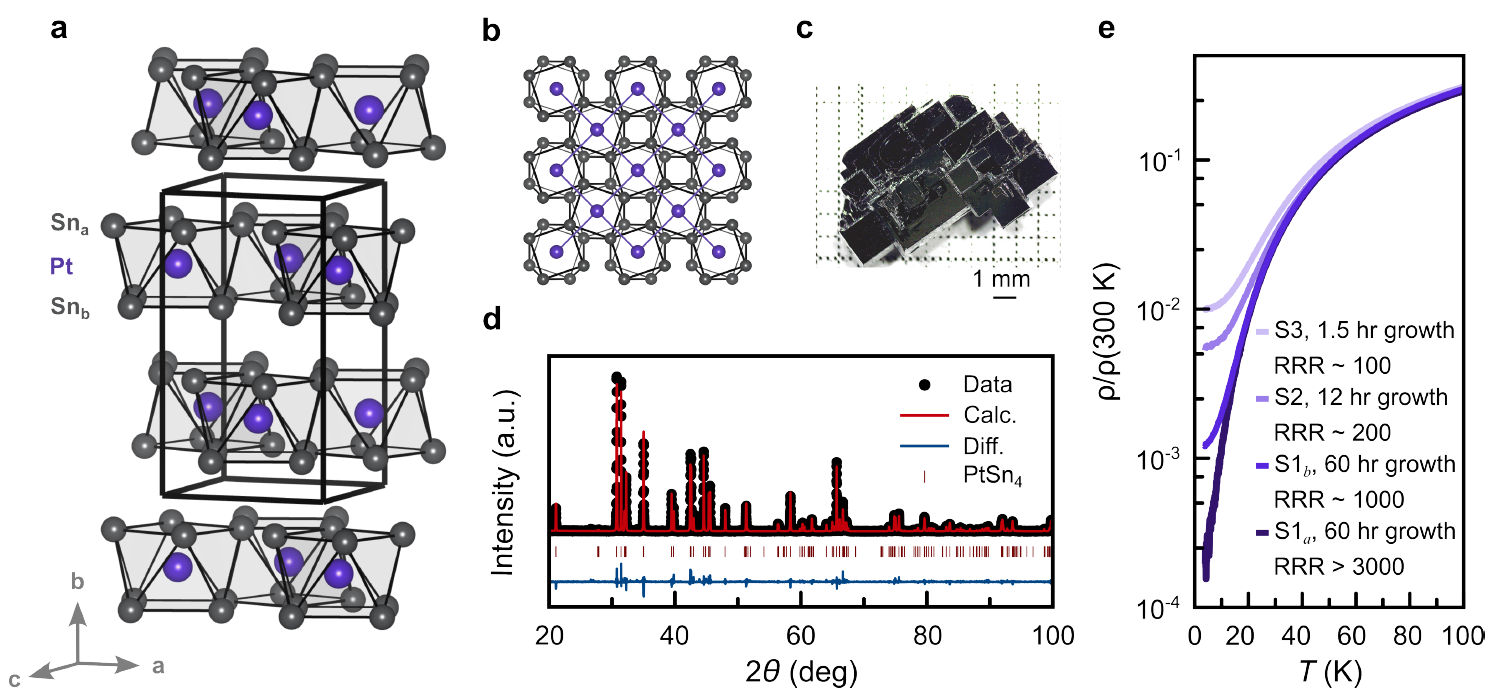
\includegraphics[width=\textwidth]{PtSn4.png}
	\caption[\textbf{Structural and transport properties of PtSn\textsubscript{4}}]{\textbf{Structural and transport properties of PtSn\textsubscript{4}}. (a,b) PtSn\textsubscript{4} adopts a quasi-two-dimensional crystal structure consisting of staggered layers, each formed by a Pt square lattice sandwiched between two Sn layers. Within each layer, square antiprismatic PtSn\textsubscript{8} units share edges, as seen along the b-axis. The two crystallographically equivalent Sn positions, Sn\textsubscript{a} and Sn\textsubscript{b}, can appear as distinct surface terminations upon cleaving. (c) The metallic self-flux method produces centimeter-scale PtSn\textsubscript{4} crystals with well-defined rectangular facets along the crystallographic b-axis. (d) Rietveld refinement of powder x-ray diffraction confirms the orthorhombic Ccca (no. 68) structure and high crystalline quality. (e) These crystals exhibit exceptionally high residual resistivity ratios (RRRs) exceeding 1000 under standard cooling conditions (60 hrs). Even with accelerated cooling (12 and 1.5 hrs), RRR values remain above 100, reflecting excellent crystalline quality and minimal defect concentration. The figure was prepared by Samikshya Sahu and is taken from an unpublished manuscript that I co-authored.}
	\label{fig:crystal_struc}
\end{figure}

\section{Sample surface Preparation}
\par Sample surface preparation is one of the keys to a successful STM experiment. As the surface of the sample is what we are trying to probe, making sure the surface is as clean and stable as possible is usually the goal of sample preparation. 

\par We achieve a clean and stable crystal surface via in-situ cleaving, it is worth mentioning that prior to the successful room-temperature cleaving, we did 2 trials of low-temperature cleaving at around 20K and the they failed, thus we will elaborate the in-situ root-temperature cleaving we performed. We first prepare the sample on bench, a mushroom like sample holder made of oxygen free copper is used. We can see a stacking structure on the left of \ref{fig:ch4_cleaves} a), from bottom to top the components are sample holder, a Pt-sheet, PtSn$_4$ single crystal, a cylindrical MACRO ceramic post. Each components are attached to the neighbors via EPO-TEK H20E, a hundred-percent solid silver-filled epoxy with low contact resistance. A polycrystalline gold is mounted next to the assembly serving as a reference metal and a tip cleaning surface. 

\par As discussed in Section 3.1, despite having a layered structure, the inter-layer bonding of PtSn$\textsubscript{4}$ is not merely weak van der Waals force, but rather metallic, making PtSn$_4$ not easily cleavable. To increase the success rate, a Pt-sheet is mounted as a buffer layer between the sample holder and the crystal. The copper sample holder has a rough surface with some residual of silver epoxy which is hard to remove, the Pt-sheets offers a cleaner interface for the epoxy polymer-network to form. And the downside of having another epoxy layer between copper sample holder and the sheet is compensated by the large Cu-Pt interface area. Therefore, cleaving on Pt-sheet gives a larger chance for a successful cleave and thus lays the foundation for the \ac{STM} experiments in this study. It is also worth mentioning that all silver epoxies are cured at the same optimal condition for good consistency. 

\begin{figure}
	\centering
	\includegraphics[width=0.8\textwidth]{Ch4_cleaving.pdf}
	\caption[\textbf{The cleaving process of PtSn\textsubscript{4}}]{\textbf{The cleaving process of PtSn\textsubscript{4}}, (a) Pre-cleaving setup of the first trial with only the S1 sample. From top to bottom: a MACRO post, the sample crystal, and a flat Pt plate, each interface bonded with EPO-TEK H20E epoxy. (b) Post-cleaving surface imaged with a K2 camera, showing large shiny regions and a central crack. (c,d) Pre-cleaving setup of the second trial with dual samples, S1 (left) and S2 (right). Two posts of different heights are used; during cleaving, the taller left post is first cleaved along the left red arrow, followed by the right post along the opposite direction to avoid contamination. (d) Post-cleaving image shows both samples with shiny flat areas and some cracks.}
	\label{fig:ch4_cleaves}
\end{figure}

\par The sample holder is then mounted to the sample plate and transferred into the preparation chamber, which sits at a pressure near $10^{-10}$ mbar and at room-temperature. We then drove one of our arms horizontally towards the downward facing sample-post assembly with directions indicated as red arrows shown in a) and c) of \ref{fig:ch4_cleaves}, the cleaving results are shown in b) and d), where we inspected the crystal in-situ with a K2 camera right after the cleave. The cleaving was successful as the cleaved crystals reveals large shiny areas. There are however, the presence of some cracks, which we avoided during the tip landing. It is worth mention that two in-situ low temperature cleaving at T\textasciitilde 20K were attempted by failed, likely because the inter-layer bonding of the crystal is stronger than the crystal-epoxy-post bonding at low temperature.

%todo: rearrange this paragrah to talk about the sample and cleaving conditions. need to modify later sections to make sure the terms are consistent. 
\par In total, our data was collected in 2 experiments on two samples with different growth conditions. While both samples used flux growth technique with the same initial stoichiometry and heating profile, their cooling rate from the highest dwelling temperature to the targeted spinning temperature is different. As shown in table \ref{table:sample}, sample S1 is cooled slowly with a rate of 4 \degree C/hr and S2 is cooled much faster at 20 \degree C/hr. A faster cooling rate generally result in an increased density of defects; the main reason being that the atoms in the crystal lattice has less time to diffuse and reorder into their lowest-energy configuration, and thus result in incomplete relaxation and trapping of defects. This is also indicated in the \ac{RRR} of two samples, where \ac{RRR} of S1 is significant higher than that of the S2. This shows S1 has a much lower level of impurity-electron scattering.
In \ac{STM} experiment, we should specify the cleaving surface as well as the sample. The first \ac{STM} experiment was performed on S1$_a$, as shown in a) of \ref{fig:ch4_cleaves}, the second experiment is on a dual sample plate, on which S1 and S2 are mounted side by side, as shown in c) of \ref{fig:ch4_cleaves}. This allows us to scan surface S1$_b$ and S2$_a$ with the same tip condition, enhancing our ability to make a better comparison.

\begin{table}[h!]
	\centering
	\begin{tabular}{|c|c|c|}
		\hline
		\textbf{Sample name} & \textbf{S1} & \textbf{S2} \\ \hline
		\textbf{Cooling rate} & 4 \degree C/hr & 20 \degree C/hr \\ \hline
		\textbf{\ac{RRR}} & 1200 & 200 \\ \hline
		\textbf{Cleaved surface} & S1\textsubscript{a}, S1\textsubscript{b} & S2\textsubscript{a} \\ \hline
	\end{tabular}
	\caption{Sample properties based on growth process and transport characteristics.}
	\label{table:sample}
\end{table}

\section{Topography overview}
\par In the course of the study of PtSn$_4$, we went through several phases, with the first phase being about the surface exploration, termination determination, scanning parameter optimization, and some spectroscopy measurements conducted on S1$_a$. The second phase was conducted on S1$_b$ and S2$_a$, with the focus on characterizing the defect scattering behaviors on both surfaces through topography and spectroscopy measurements. This section will cover the topographical aspect of this study. 

\begin{figure}
	\centering
	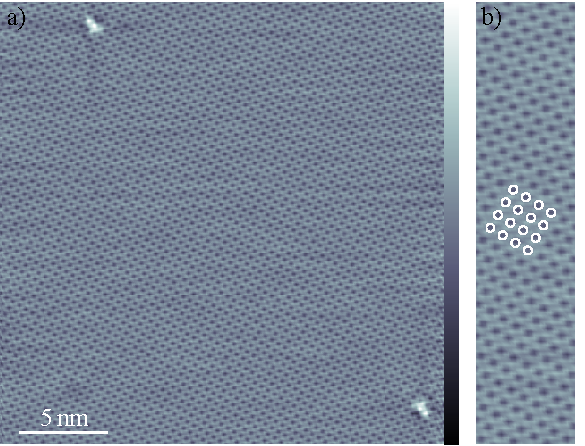
\includegraphics[width=\textwidth]{Ch4_Pristine_PtSn4.pdf}
	\caption[\textbf{Pristine topography on PtSn\textsubscript{4}}]{\textbf{Pristine topography on PtSn\textsubscript{4}}(a)Typical STM topography of PtSn$_4$, characterized by waffle-like square corrugations and sparse defects at different atomic sites. (b) Overlay of the Pt layer on the topography, which aligns perfectly with the observed square corrugations.}
	\label{fig:ch4_pristinetopo}
\end{figure}

\par In total, we took over 20000 STM topographies in this study, covering an area of over two million nanometer squared. More specifically, we acquired around 10000 images on 5 macroscopic spots on the S1$_a$ surface, around 5000 images on the S1$_a$ surface, and around 2000 images on 2 macroscopic spots on the S2$_a$ surface. 
Panel a) of \ref{fig:ch4_pristinetopo} exhibits a typical STM topography on PtSn$_4$, it is featured by waffle-like square corrugations and sparse defects at different atomic sites. Pristine cleaved surfaces are remarkably defect free, which we quantify through a careful statistical analysis in a subsequent section. We can overlay the Pt-layer to the surface of the pristine surface as shown in b) of \ref{fig:ch4_pristinetopo} and it maps perfectly with the square corrugations we observed. It might be tempting to say that we are typically scanning on the Pt-surface, but note that as mentioned in Ch.2, the tunneling current of STM has both the contribution of distance and electronic structure of the sample, the pattern revealed on topography is not necessarily the top most surface. To determine on what termination we are scanning, we ran a full terrace characterization.


\subsection{Terrace determination}
%todo: to insert the pdf showing potential cleavin9g planes of PtSn4.
\par Topographies of PtSn$_4$ reveal flat terraces that belong to different cleavage planes. Inspecting the crystal structure of PtSn$_4$, we note that there are three possible cleavage planes as shown in Fig 2. They are Sn$_a$-Pt, Pt-Sn$_b$, and Sn$_b$-Sn$_a$. Sn$_b$-Sn$_a$ bond has twice the length as Sn$_a$-Pt and Pt-Sn$_b$ bond and thus is weaker. We expect this material to cleave predominately between Sn$_b$-Sn$_a$. 

\begin{figure}
	\centering
	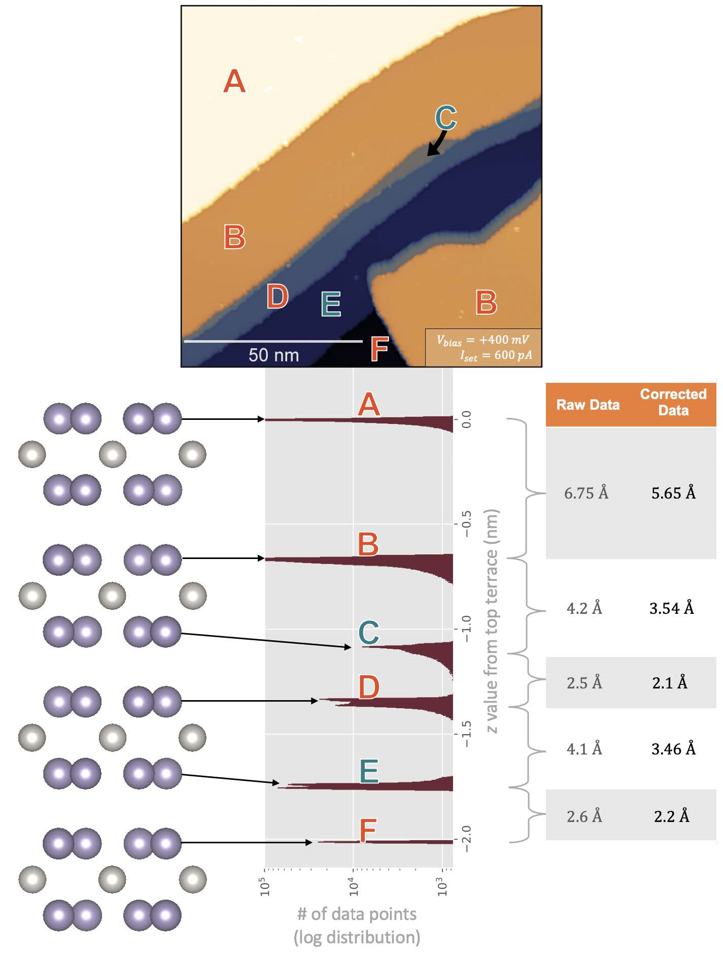
\includegraphics[width=\textwidth]{Ch4_termination.png}
	\caption[\textbf{Termination analysis of PtSn\textsubscript{4} surfaces}]{\textbf{Termination analysis of PtSn\textsubscript{4} surfaces}.Top: STM topography showing multiple terraces labeled A–F, corresponding to distinct cleavage terminations.
	Bottom: Histogram of step heights measured relative to the top terrace, aligned with structural models of candidate terminations. Both raw and corrected step-height values are listed. The figure is adopted from reference \cite{warnerDefectTerraceCharacterization2022}}
	\label{fig:ch4_termination}
\end{figure}

\par In the experiment, we often landed our tips on a dominating terrace that is big and flat, and by scanning the step edges of the terraces, we could also see other terminations but with much less occurrence. To determine the dominating terrace we are scanning, we analyzed the step heights on a step-edge area, as shown in \ref{fig:ch4_termination}. 

Before discussing the result shown in panel (b) of Figure \ref{fig:ch4_termination}, it is useful to recall how cleaving modifies the sample structure. Cleaving breaks the translational symmetry of the crystal, with the strongest effect on the surface layer. Here, the covering layers are replaced by vacuum, and without their support the surface atoms “relax” inward. This relaxation reduces the distance between the topmost layer and the layer beneath it compared to the bulk lattice spacing. The extent of this relaxation depends on the cleavage plane and its local bonding environment.

In PtSn$_4$, there are two possible Sn-terminated surfaces. If the surface ends at an Sn$_a$ layer (from an Sn$_b$–Sn$_a$ cleave), the relaxation is relatively small. In contrast, if the surface ends at an Sn$_b$ layer (from a Pt–Sn$_b$ cleave), the relaxation is stronger. As a result, the apparent step height between Sn$_a$ and Sn$_b$ terminations is expected to differ from the bulk lattice spacing of 2.8{\AA} (one-quarter of the unit cell along the $b$-axis): it will appear larger than 2.8{\AA} for an Sn$_a$–Sn$_b$ step, and smaller than 2.8{\AA} for an Sn$_b$–Sn$_a$ step.This prediction matches the step-height profiles we measured, shown in panel (b) of Figure \ref{fig:ch4_termination}. The height histogram extracted from the topography displays distinct peaks corresponding to different terminations. From this analysis, we conclude that the vast majority of the surface is Sn$_a$-terminated. Other terminations, corresponding to the Pt or Sn$_b$ layers, were rare, accounting for less than 1\% of the total scanned area.


\par For more details of the termination determination of PtSn$_4$, the reader can consult chapter 3 of Ashley Warner's thesis \cite{warnerDefectTerraceCharacterization2022}.



\section{Defect Analysis}
Defects play a central role in determining the low-temperature transport properties of a material. At cryogenic temperatures, electron-phonon and electron-electron scattering are strongly suppressed, leaving electron-defect scattering as the dominant contribution to the residual resistivity. A detailed characterization of the real-space features, spectroscopic signatures, and densities of existing types of defect is therefore essential to understand the microscopic origin of electron scattering in this system.

In this section, we combine high-resolution STM topography, defect-specific spectroscopy, and statistical analysis to build a comprehensive picture of the defect landscape in PtSn\textsubscript{4}. Topographic imaging allows us to classify defects by lattice site and local symmetry. Spectroscopy provides insight into how different defects perturb the local density of states, distinguishing weak perturbations at Pt sites from stronger modifications at Sn sites. Finally, a statistical framework enables quantitative estimates of defect densities and their correlation with transport properties across samples of different crystalline quality. Together, these complementary approaches clarify the intrinsic and extrinsic contributions to scattering and establish the role of defects in governing the exceptional residual resistivity ratio of PtSn\textsubscript{4}.

\begin{figure}
	\centering
	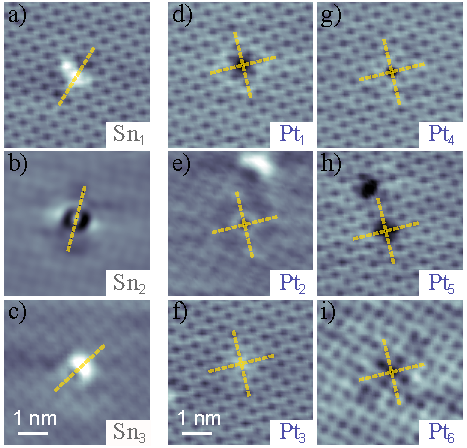
\includegraphics[width=\textwidth]{Ch4_defect_gallery.pdf}
	\caption[\textbf{Gallery of nine distinct defect types identified in PtSn\textsubscript{4}}]{\textbf{Gallery of nine distinct defect types identified in PtSn\textsubscript{4}}: (a–c) three Sn-site defects and (d–i) six Pt-site defects. The black lines mark the corresponding mirror planes of each defect. STM images were acquired under varying tunneling conditions: (a, d, f, g, h) at –400 meV, 500 pA; (b) at +400 meV, 600 pA; (c) at –400 meV, 600 pA; (e) at –500 meV, 500 pA; and (i) at –400 meV, 500 pA. All measurements were conducted at 4.4 K.}
	\label{fig:ch4_defectgallery}
\end{figure}

\subsection{Defects Topography}
Throughout the exploration on both fast-cooled and slow-cooled sample, different types of defects are observed, with the dominating source being point defects. In total, we observed 9 types of point defects in PtSn$_4$ as shown in Figure. \ref{fig:ch4_defectgallery}. 6 types are characterized as reside on Pt-sites and 3 on the Sn-site. Whether the defect belongs to a Sn-site or a Pt-site is determined with the lattice symmetry preserved in the Pt-layer and Sn-layer. As shown in Figure. \ref{fig:ch4_symmetry}, point defects sitting at the Pt-site will break the local translational symmetry, it changes the local electronic environment of 4 neighboring Pt atoms and thus exhibits a 2 fold symmetry and mirror symmetry in 2 axes(C$_2v$). As for Sn-layers, a modification on the Sn-site will result in a pattern with lower symmetry, with mirror symmetry in only 1 axis. Therefore, we can determine the what plane a defect lies in, based on the symmetry exhibited by the defect topography. 

\begin{figure}
	\centering
	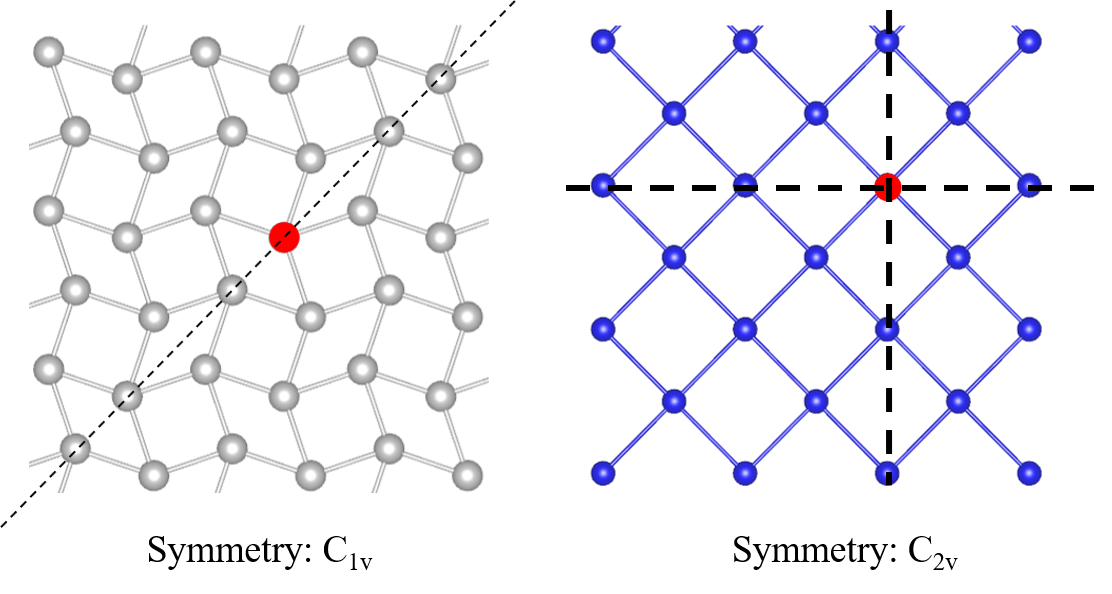
\includegraphics[width=\textwidth]{Ch4_symmetry.png}
	\caption[\textbf{Symmetry of a point defect on Sn and Pt layer}]{\textbf{Symmetry of a point defect in Sn and Pt layer}. Left: Sn-layer defect with preserved C\textsubscript{1v} mirror symmetry. Right: Pt-layer defect with preserved C\textsubscript{2v} symmetry.}
	\label{fig:ch4_symmetry}
\end{figure}


\subsection{Defect Spectroscopy}\label{section:defect_spectro}
To investigate the local electronic response of individual defects in PtSn\textsubscript{4}, we performed spatially resolved scanning tunneling spectroscopy (STS) across six distinct defect types observed in both slow- and fast-cooled samples. Figure \ref{fig:defect_spectro} summarizes the results, combining structural topographies, defect-centered spectra, and reference pristine spectra.

The top row of Fig. \ref{fig:defect_spectro} (panels a–d) presents representative STM topographies of three Sn-site (Sn1, Sn2, Sn3) and three Pt-site (Pt1, Pt2, Pt3) defects. The second row (panels e–h) shows $dI/dV$ spectra acquired directly on defect centers and in their vicinity, together with a pristine reference spectrum extracted from the same scan. Because of the sparse distribution of defects in PtSn\textsubscript{4}, no single field of view contained all defect types; instead, four independent scans were used. To account for variations in junction conditions between scans, pristine reference spectra were taken from each corresponding dataset and serve as the baseline for comparison. The third row (panels i–l) displays sets of pristine spectra acquired from defect-free regions, with individual traces in faint blue and their average in black. Three recurring spectral features near the Fermi level are highlighted by vertical colored markers: a shoulder feature at $\sim$250 meV (green), followed by a steep rise, and two dominant peaks at $\sim$300 meV (cyan) and $\sim$450 meV (purple).

Spectroscopic signatures at Pt-site defects show only modest deviations from the pristine response. As illustrated in panels e) and f), all three characteristic spectral features remain visible, and their relative energies are unchanged. The most notable effect is a suppression of the overall spectral weight, typically in the range of 10–25\% compared to pristine regions. This indicates that Pt-site defects perturb the local density of states (LDOS) only weakly, acting potentially only as minor scattering centers.

By contrast, Sn-site defects produce far more substantial modifications of the LDOS. For the Sn1 defect, the low-energy shoulder shifts toward lower bias by approximately 50 meV, and the $\sim$300 meV peak is strongly suppressed or absent altogether. The higher-energy $\sim$450 meV peak persists but with an overall reduction in intensity of about 50\%. The Sn2 defect exhibits an even more striking spatial variation: spectra taken directly at the defect center show an $\sim$80\% suppression of the intensity peak, while spectra taken at the lobes surrounding the defect closely resemble the pristine surface. For the Sn3 defect, the shoulder region is enhanced, the $\sim$300 meV peak remains nearly unchanged, and the $\sim$450 meV peak is absent. These diverse responses among Sn-site defects highlight their ability to reshape the local electronic environment in distinct ways.

In summary, the spectroscopy reveals two main effects. First, no distinct defect-bound states are detected within the stable energy window; instead, defect-centered spectra largely preserve the pristine LDOS features, with modifications limited to overall intensity. Second, Sn-site and Pt-site defects exhibit different degrees of LDOS modulation: Pt-site defects cause only mild suppression of spectral weight, while Sn-site defects shift or suppress characteristic features and display strong spatial variation. The weak perturbation from Pt-site defects is consistent with the observed defect intolerance and high carrier mobility of PtSn\textsubscript{4}, whereas the stronger LDOS modifications from Sn-site defects suggest they may represent the dominant source of electron scattering when present.

However, as noted in Appendix \ref{appen:non-intrinsic}, certain Sn-site features—such as the Sn1 defect—may have non-intrinsic origins. This distinction underscores the importance of considering both intrinsic and extrinsic contributions when interpreting defect statistics.

\begin{figure}
	\centering
	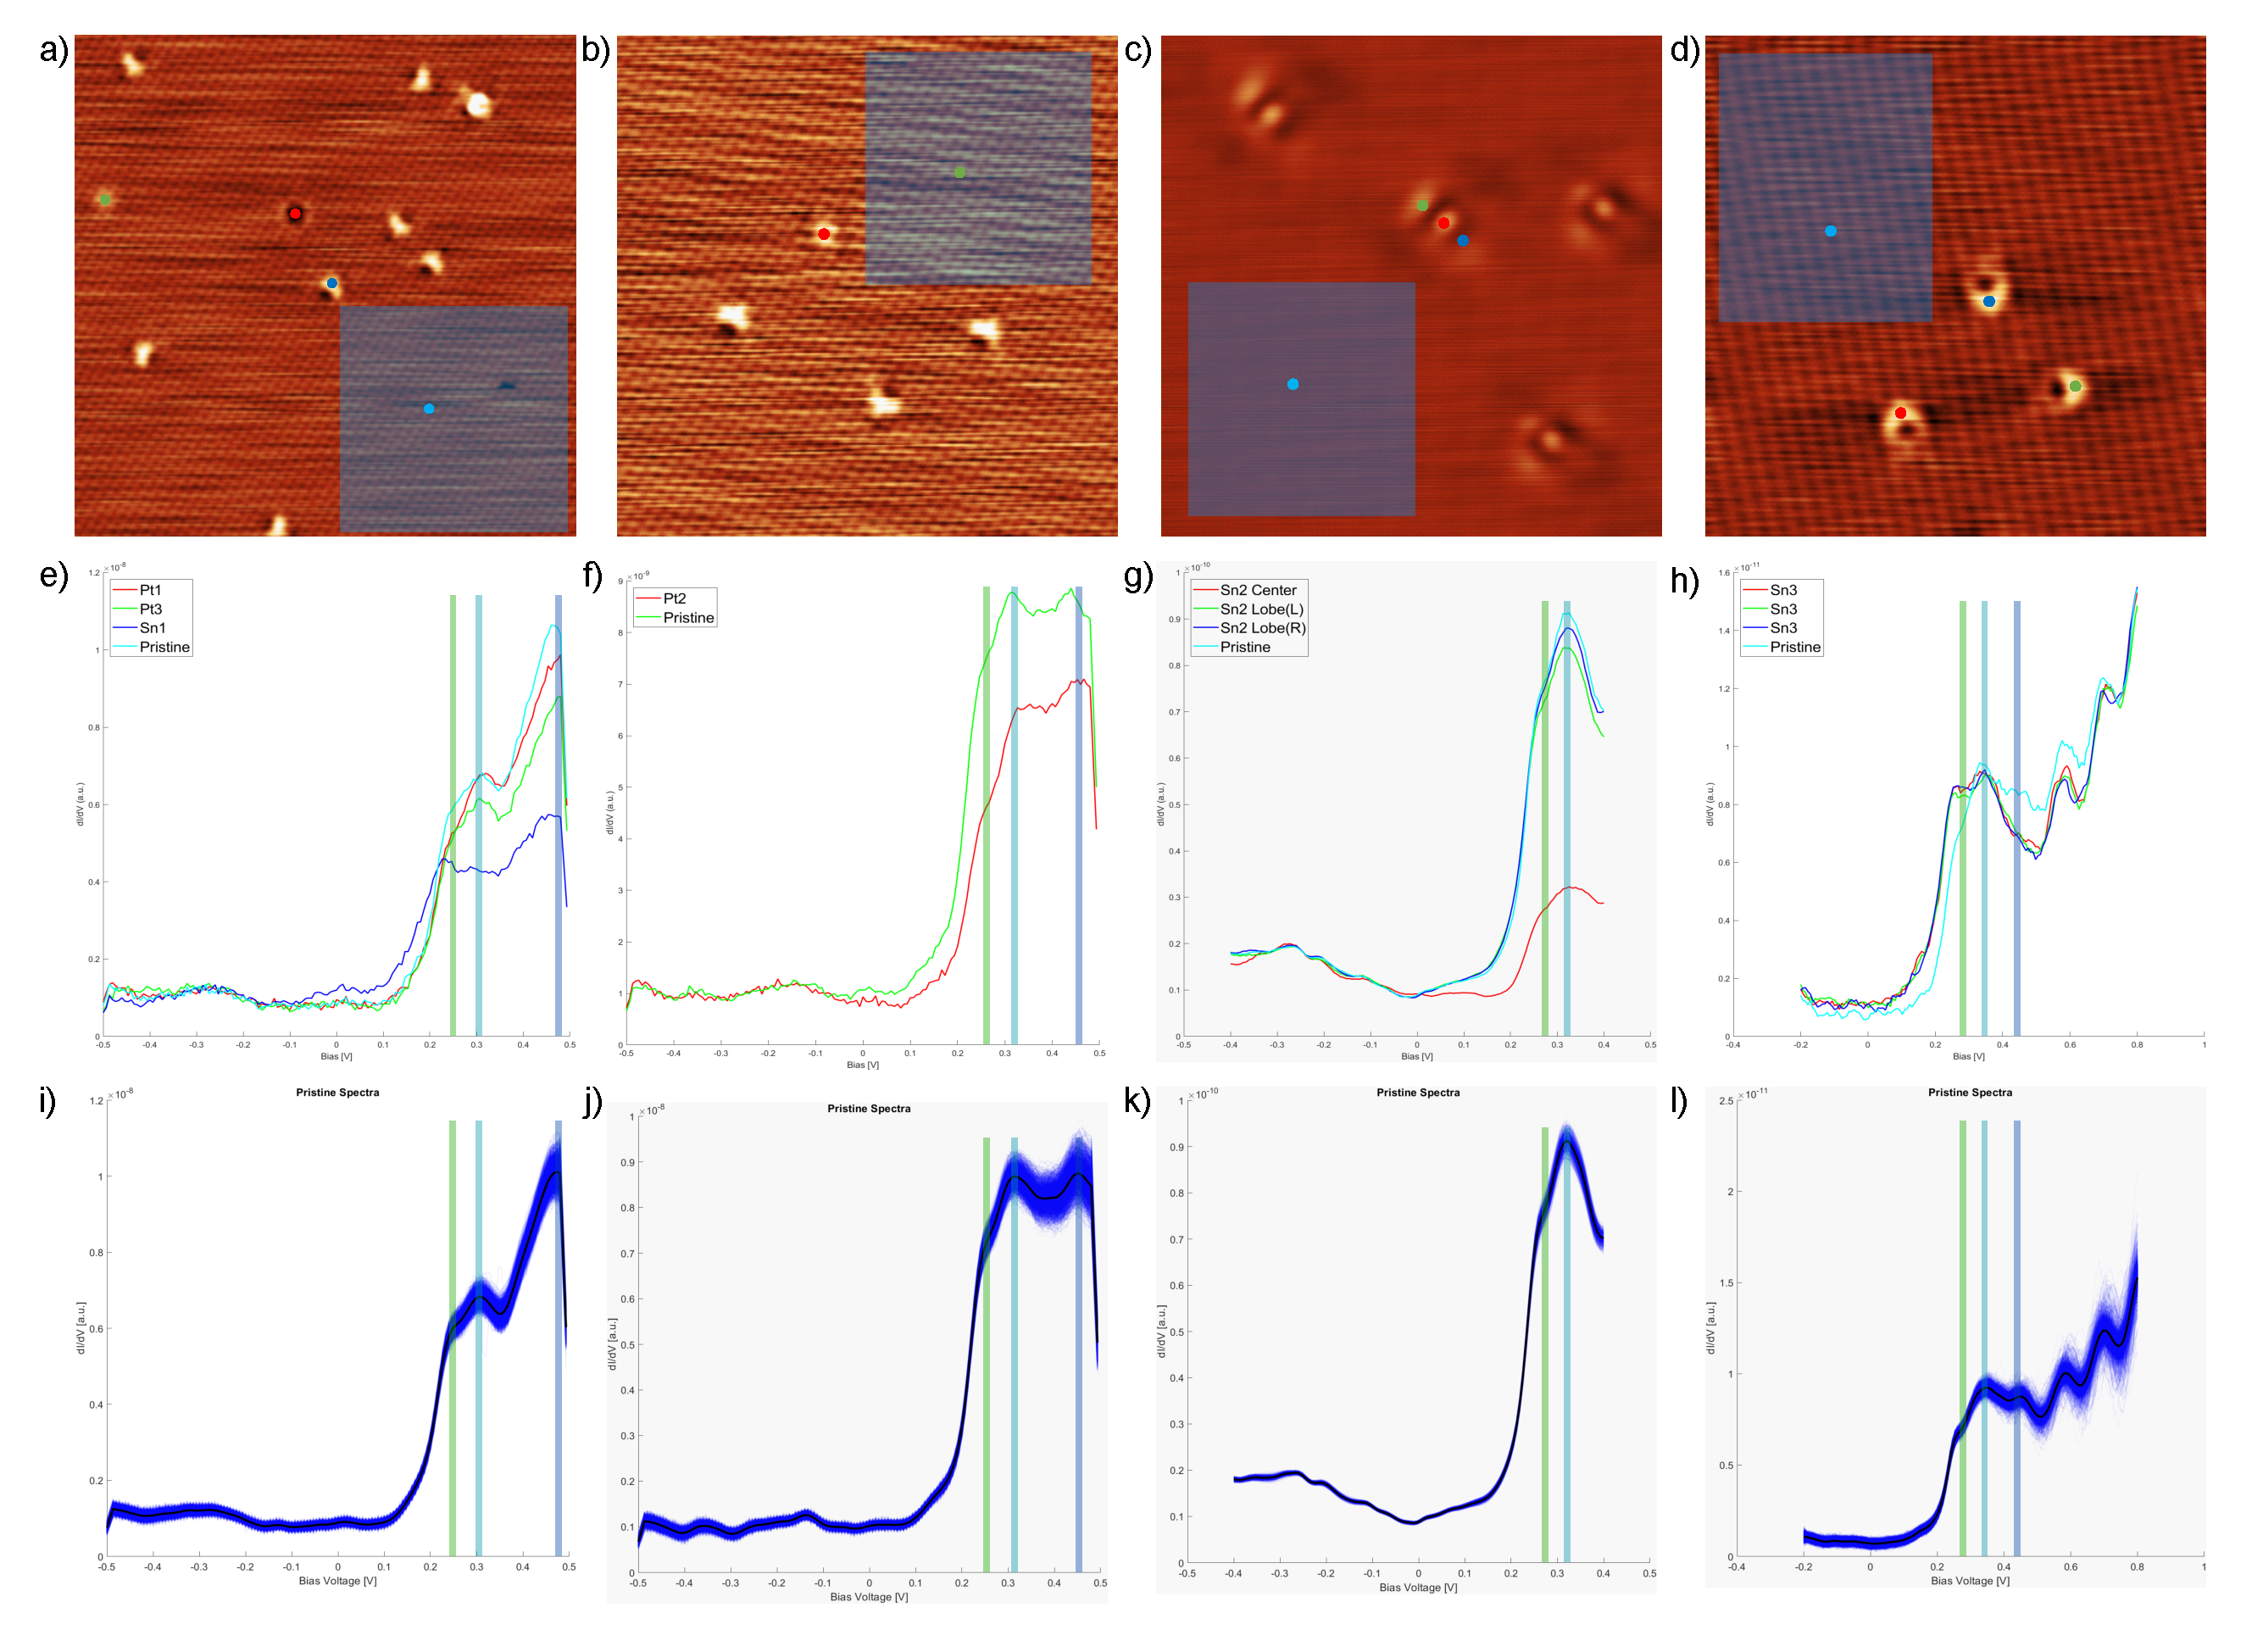
\includegraphics[width=\textwidth]{defect_specs_ALL.pdf}
	\caption[\textbf{Defect-specific spectroscopy in PtSn\textsubscript{4}}]{\textbf{Defect-specific spectroscopy in PtSn\textsubscript{4}}:
		(a–d): STM topographies of six distinct defect types (Sn1, Sn2, Sn3, Pt1, Pt2, Pt3) observed across fast- and slow-cooled PtSn\textsubscript{4} samples.
		(e–h): Spatially resolved dI/dV spectra taken at and around each defect, with a reference pristine spectrum from the same scan. Overall density suppression and partial suppression of spectral features are presented on different defect centers; However, distinct defect states close to the Fermi level are not observed. All measurement locations are marked in the topographies above.
		(i-l): Pristine spectra extracted from blue-boxed regions in the topographies. Individual spectra are shown in faint blue; their average is plotted in black. Three characteristic spectral features near the Fermi level are highlighted by vertical colored lines.}
	\label{fig:defect_spectro}
\end{figure}

\subsection{Defect Statistics}

\subsubsection{Statistical Framework}
Defect density is a direct metric to evaluate the level of lattice perfection of a system. To achieve a reliable defect density and their associated undertainties, we used a statistical framework grounded in binomial and Poisson distribution principles, and justify its applicability to our experimental observations.
\par Our analysis of defect densities in PtSn\textsubscript{4} crystals commences with the consensus that that point defects emerge as a stochastic process\cite{rudolphDefectFormationCrystal2010},\cite{mosquera-loisImperfectionsAreNot2023}. Given the crystal lattice structure, defects can randomly occur at any site, rendering each occurrence an independent event. This randomness and independence are fundamental assumptions that underpin our methodological approach, it is justified by STM topography as mentioned in the later paragraph.  
\par In total, 3 types of Sn-site defects and 6 kinds of Pt defects are observed. Since each site can only be occupied by one defect, to individual types of defect, we can conceptualize each lattice site as a discrete trial within a binomial framework. A 'success' in this context was defined as the presence of this particular type of point defect at a given site, denoted by '1', while its absence was considered a 'reference event', denoted by '0'. This binary scheme facilitated the application of the binomial distribution to model the statistics of defect occurrences across the lattice.
\par Given the extensive scanning area corresponding to a vast number of lattice sites (trial), coupled with the markedly low probability of defect occurrence (success rate), our analysis necessitated an approximation to simplify computations and enhance analytical tractability. The 
binomial distribution converges to the Poisson distribution under these conditions of large trial numbers and a small success rate. This approximation is underpinned by established statistical criteria. When the number of trials (n) exceeds 100 and the success rate (p) is below 0.1, the Poisson distribution serves as an effective surrogate for the binomial distribution. 
\par In our specific case, with n on the order of $10^5$ and p ranging between $10^{-3}$ and $10^{-5}$, the mean of the Poisson distribution ($\lambda=n\cdot p$) falls between 1 and 100. These are the conditions where the Poisson approximation is not only justified but advantageous, facilitating a more streamlined analysis of defect densities.
\par The sparse and non-clustered distribution of defects, as revealed through Scanning Tunneling Microscopy (STM) topographies, provided empirical validation for our methodological choices. The lack of defect clustering corroborates the assumption of defect occurrences as independent events, likely driven by thermal activation rather than mechanical strain. Mechanical strain would predictably induce clustering or patterned distributions of defects due to stress relaxation dynamics within the crystal lattice.
\par The transition from a binomial to a Poisson framework is further justified by the nature of our observations and the computational efficacy it offers. The Poisson distribution, known for its applicability to rare events in large populations, aligns well with the characteristics of defect formation in PtSn4 crystals. This alignment not only simplifies the mathematical treatment of defect statistics but also enhances the interpretability of our findings.

\subsubsection{Defect counting}
Defect counting is one of the key components to this study. Before the labour work of manually counting the defects, it is important to sample our image pool to avoid bias and enhance statistical representativeness. There are a few principles I followed with image selection: 
\begin{itemize}
	\item 1. Use images with good and consistent tip conditions(here the standard is whether the tip can image atomic resolution), but images taken at different bias voltages are allowed. 
	\par Rationale: Defects images taken by consistent tip conditions will give a more consistent pattern and thus more robust counting.	
	\item 2. Avoid repetitive areas. 
	\par Rationale: Many of the images are take on the same area to gauge the tip conditions.
	\item 3. Choose big size images, here we use images of size bigger than 50nm by 50nm.
	\par Rationale: Smaller size images are usually taken to focus on object of interest, thus biased.  
\end{itemize}  
Just to give the reader a sense, we collected around 20000 topographic images in our study, after standard 1, we are left with around 3000 images, then we apply standard 2, we again eliminate about 80\% of the images, and with standard 3, we are left with in total 55 images, with 33 on sample S1 and 22 on sample S2. However, with the statistical framework we established in last section, the areas covered by these images are still big enough for us to make statistically meaningful claim on defect density.

\subsubsection{Defect density}

\begin{table*}
		\renewcommand{\arraystretch}{1.5}  % Increased line separation
		\caption{Defect statistics of two samples of PtSn$_4$ grown at two different cooling rates: slow-cooled sample S1 (\ac{RRR}~$>1000$) and fast-cooled sample S2 (\ac{RRR}~$=200$).} \label{tab:table1}
		\begin{tabular}{ccccc}
			Defect & Symmetry & Category & $\rho A_{\text{S1}}$ (per unit cell) & $\rho A_{\text{S2}}$ (per unit cell) \\ 
			\hline
			Sn$_1$ (Croissant)\footnote{This kind of defect is believed to be non-intrinsic} & $C_{1v}$ & Sn site & $1.00(0.02) \times 10^{-3}$ & $3.50(0.03) \times 10^{-3}$ \\
			Sn$_2$ (Spearhead)$^{\text{a}}$ & $C_{1v}$ & Sn site & $1.46(0.02) \times 10^{-3}$ & $0.216(0.008) \times 10^{-3}$ \\
			Sn$_3$ (Crescent)$^{\text{a}}$ & C$_{1v}$ & Sn site & $1.545(0.007) \times 10^{-4}$ & $0.033(0.009) \times 10^{-4}$ \\
			\hline
			Pt$_1$ & $C_{2v}$ & Pt site & $2.9(0.5) \times 10^{-5}$ & $5.6(0.4) \times 10^{-5}$ \\
			Pt$_2$ & $C_{2v}$ & Pt site & $3.8(0.5) \times 10^{-5}$ & $5.4(0.4) \times 10^{-5}$ \\
			Pt$_3$ & $C_{2v}$ & Pt site & $1.7(0.3) \times 10^{-5}$ & $2.1(0.3) \times 10^{-5}$ \\
			Pt$_4$ & $C_{2v}$ & Pt site & $2.8(0.4) \times 10^{-5}$ & Not Observed \\
			Pt$_5$ & $C_{2v}$ & Pt site & Not Observed & $2.0(0.2) \times 10^{-5}$ \\
			Pt$_6$ & $C_{2v}$ & Pt site & Not Observed & $0.5(0.1) \times 10^{-5}$ \\
			\hline
			Sn$_{\text{total}}$ &  &  & $2.61(0.03) \times 10^{-3}$ & $3.72(0.03) \times 10^{-3}$ \\
			Pt$_1$+Pt$_2$+Pt$_3$ &  &  & $0.84(0.08) \times 10^{-4}$ & $1.31(0.06) \times 10^{-4}$ \\
			Pt$_{\text{total}}$ &  &  & $1.1(0.08) \times 10^{-4}$ & $1.56(0.07) \times 10^{-4}$ \\
		\end{tabular}
\end{table*}

\par Defect densities for each type are reported in Table~\ref{tab:table1}. defect densities are reported on both the highRRR and lowRRR sample. Pt site defects are significantly rarer than Sn site defects, as discussed below. Of the 6 types of Pt-site defects, Pt$_{1}$,Pt$_{2}$ and Pt$_{3}$ were observed in both samples. All Pt site defects are in the range of 10--50 ppm, and of the three types present in both high and lower RRR samples, all increase in the fast-cooled lower RRR sample. The overall density of Pt site defects increases for the lower RRR sample, consistent with expectations from the increased low-temperature resistivity originating from point defect scatterers.

\par Defects residing on the Sn site are more prevalent in both samples, having densities that are between one and two orders of magnitude larger than the Pt site defects. However, the analysis is confounded by sensitivity to surface effects. Although significant increases in defects over time due to the adsorption of contaminants were not observed, other extrinsic variability appears to significantly influence the total Sn site defect density. In particular, the Sn$_1$ (croissant) defect is readily induced by the tip through voltage pulses or prolonged high voltage, and these defects have been observed to move and even annihilate, leading us to suspect these defects correspond to a Frenkel pair (a Sn adatom-Sn vacancy pair). The Sn$_2$ and Sn$_3$ defects anomalously decrease in S2 , contrary to expectations from the transport measurements. We suspect these correspond to vacancies and/or adatoms that arise during cleaving, as the Sn surface is easily disturbed. With these extrinsic factors in mind contributing to the total observed defect density, we can only place an upper limit on the number of scattering sites. While intrinsic Sn site defects are surely present, they are dominated by extrinsic ones, we will therefore focus more on the Pt site defects.

\par Having established that the Pt site defects provide a more reliable indicator of the intrinsic defect concentration, we can next examine the differences between sample S1 and S2. Pt$_1$, as the dominant intrinsic defect, doubled in S2, and the Pt$_2$ defect also has a sizable increase in the S2. And Pt$_3$ does not have a notable change in the density. Taken in aggregate the increase in defects corresponds to a $1.5\times$ larger concentration of Pt site defects in S2 with a lower \ac{RRR} as compared to S1 with a higher \ac{RRR}.  The increase in intrinsic defect densities is aligned with the increase in the low-temperature resistivity across the two samples. 
%todo: Need revisit. after analysis of QPI in PtSn4 for different defects, I can maybe then claim the scattering rate of different defects differ little, and thus, we can correlate e-i scattering directly to defect density.
Note that electron-impurity scattering is contributed by both the density of different types of defects and their scattering strength, however, as shown by the \ac{QPI} analysis in Ch.6, the scattering strength of different defect types differ little, we could expect a linear correlation between defect concentration and residual resistivity due to electron-defect scattering. The observed increase of $1.5$ times in the Pt site defects described here fails to account for the $5\times$ decrease in the \ac{RRR} value for S2 as compared to S1. We therefore conclude that, although the Sn site defects are dramatically obscured by the non-intrinsic effects described above, they must account for the majority of increased scattering centers. 


\section{Conclusion}
In this chapter, we established a statistical framework to quantify defect populations in PtSn\textsubscript{4} using multinomial statistics on STM topographies. By distinguishing between Pt- and Sn-site defects and systematically comparing multiple samples under different growth conditions, we found that the defect densities are exceptionally low—even under rapid cooling. This places PtSn\textsubscript{4} among the most defect-free semimetals studied to date.

The implications of such dilute defect populations are twofold. On a methodological level, the ability to resolve defect-specific densities provides a microscopic metric for benchmarking crystal quality. On a physical level, the scarcity of scattering centers naturally accounts for the vanishing residual resistivity and exceptionally high residual resistivity ratio (RRR) reported in transport studies. This interpretation points to crystalline perfection, rather than exotic topological suppression of scattering; in line with the semi-classical transport models established to address the origin of the extreme magnetoresistance in PtSn\textsubscript{4}\cite{diazSemiclassicalOriginExtreme2024}. To conclude, the statistical analysis of defect-specific populations not only underscores the intrinsic quality of PtSn\textsubscript{4}, but also reframes its remarkable transport properties in terms of lattice perfection, with topological effects playing at most a secondary role. 